% Copyright 2018 Melvin Eloy Irizarry-Gelpí
\chapter{Impulse and Momentum}
%%%%%%%%%%%%%%%%%%%%%%%%%%%%%%%%%%%%%%%%%%%%%%%%%%%%%%%%%%%%%%%%%%%%%%%%%%%%%%%%
...
%%%%%%%%%%%%%%%%%%%%%%%%%%%%%%%%%%%%%%%%%%%%%%%%%%%%%%%%%%%%%%%%%%%%%%%%%%%%%%%%
\section{Preliminary}
%%%%%%%%%%%%%%%%%%%%%%%%%%%%%%%%%%%%%%%%%%%%%%%%%%%%%%%%%%%%%%%%%%%%%%%%%%%%%%%%
Linear momentum (or just \textbf{momentum}) is a physical quantity that incorporates velocity and mass:
\begin{equation}
    p = m v
\end{equation}
Due to the second law of motion, a net \textbf{force} causes an acceleration (a change in the velocity of an object). This in turn leads to a change in the momentum of an object. The precise relationship between momentum and forces includes a quantity called \textbf{impulse}.

Formally, impulse is defined as the area under the curve in a \textbf{force versus time} graph. In principle, we need calculus to find the area under a curve. In practice we use a simple approximation: we approximate the curve as a \textbf{flat line}. The area under a flat line has the same shape as a rectangle. The area of a rectangle is the length multiplied by the width. Which flat line to use? Since force is in the vertical axis, a flat horizontal line corresponds to a fixed value of force along time. An appropriate choice for the fixed value is the \textbf{time-averaged force} $\bar{F}$. This would correspond to the width of the rectangle. The length of the rectangle is the amount of time $\Delta t$ that the force acts. The ``area'' is thus given by
\begin{equation}
    \text{``area'' } = \bar{F} \times \Delta t = \text{ impulse}
\end{equation}
Impulse has units of force multiplying time. If force is in newtons (N) and time in seconds (s), then impulse has units of N s. However, the newton is equivalent to
\begin{equation}
    1 \text{ N} = 1 \text{ kg m/s}^{2}
\end{equation}
Thus, the N s is equivalent to
\begin{equation}
    1 \text{ N s} = 1 \text{ kg m/s}
\end{equation}
If you look carefully, these are the same units of momentum. This does not mean that impulse is the same as momentum. Indeed, impulse can also be defined as the \textbf{change in momentum}:
\begin{equation}
    \text{impulse } = p_{2} - p_{1}
\end{equation}
%%%%%%%%%%%%%%%%%%%%%%%%%%%%%%%%%%%%%%%%%%%%%%%%%%%%%%%%%%%%%%%%%%%%%%%%%%%%%%%%
\section{Experiment}
%%%%%%%%%%%%%%%%%%%%%%%%%%%%%%%%%%%%%%%%%%%%%%%%%%%%%%%%%%%%%%%%%%%%%%%%%%%%%%%%
In order to verify the relationship between momentum, force, and impulse, we need to use a mechanical system where momentum and force change with time. A cart, moving along a track and colliding with a force sensor is perfect for this. Different attachment on the force sensor allow us to study different kinds of collisions. We also use a photogate to measure the speed of the cart before and after the collision. In this way, we collect data on force, and momentum, and the impulse can be determined in two different ways.
%%%%%%%%%%%%%%%%%%%%%%%%%%%%%%%%%%%%%%%%%%%%%%%%%%%%%%%%%%%%%%%%%%%%%%%%%%%%%%%%
\section{Analysis}
%%%%%%%%%%%%%%%%%%%%%%%%%%%%%%%%%%%%%%%%%%%%%%%%%%%%%%%%%%%%%%%%%%%%%%%%%%%%%%%%
We are going to determine the amount of impulse in two different ways.
%%%%%%%%%%%%%%%%%%%%%%%%%%%%%%%%%%%%%%%%%%%%%%%%%%%%%%%%%%%%%%%%%%%%%%%%%%%%%%%%
\subsection{Impulse from Change in Momentum}
%%%%%%%%%%%%%%%%%%%%%%%%%%%%%%%%%%%%%%%%%%%%%%%%%%%%%%%%%%%%%%%%%%%%%%%%%%%%%%%%
The photogate measures the velocity of the object before the collision ($v_{1}$) and after the collision ($v_{2}$). Strictly speaking, \textbf{one of the velocities value should be negative} because there is \textbf{a change in the direction} of motion. We are going to multiply the value for $v_{2}$ by $-1$ in order to \textbf{make it negative}.

With the values of velocity, and the mass of the object, you can find the momentum of the object before the collision,
\begin{equation}
    p_{1} = m v_{1}
\end{equation}
and the momentum after the collision,
\begin{equation}
    p_{2} = m v_{2}
\end{equation}
The change in momentum is
\begin{equation}
    \Delta p = p_{2} - p_{1}
\end{equation}
This is the first estimate of the amount of impulse during the collision.
%%%%%%%%%%%%%%%%%%%%%%%%%%%%%%%%%%%%%%%%%%%%%%%%%%%%%%%%%%%%%%%%%%%%%%%%%%%%%%%%
\subsection{Impulse from Force Acting Over Time}
%%%%%%%%%%%%%%%%%%%%%%%%%%%%%%%%%%%%%%%%%%%%%%%%%%%%%%%%%%%%%%%%%%%%%%%%%%%%%%%%
The force sensor measures the amount of force on the sensor during the collision. First you need to determine when the collision is taking place. This involves making a force versus time graph and finding the time $t_{1}$ when the collision begins and the time $t_{2}$ when it ends. With these times you can compute the amount of time that the collision lasts:
\begin{equation}
    \Delta t = t_{2} - t_{1}
\end{equation}
Then you delete all the force values before and after the collision in the force column. Finally, you can compute the average force during this time period. This gives you the value of $\bar{F}$. With $\bar{F}$ and $\Delta t$ you can compute the impulse:
\begin{equation}
    \text{impulse } = \bar{F} \times \Delta t
\end{equation}
This is the second estimate of the amount of impulse during the collision.
%%%%%%%%%%%%%%%%%%%%%%%%%%%%%%%%%%%%%%%%%%%%%%%%%%%%%%%%%%%%%%%%%%%%%%%%%%%%%%%%
\section{My Data}
%%%%%%%%%%%%%%%%%%%%%%%%%%%%%%%%%%%%%%%%%%%%%%%%%%%%%%%%%%%%%%%%%%%%%%%%%%%%%%%%
There are two experiments: elastic and inelastic collisions. The difference between these experiment is that in the inelastic case, the amount of force during the collision is larger, and the velocity (and momentum) after the inelastic collision is zero. Besides that, the analysis is almost identical.
%%%%%%%%%%%%%%%%%%%%%%%%%%%%%%%%%%%%%%%%%%%%%%%%%%%%%%%%%%%%%%%%%%%%%%%%%%%%%%%%
\subsection{Elastic Collision}
%%%%%%%%%%%%%%%%%%%%%%%%%%%%%%%%%%%%%%%%%%%%%%%%%%%%%%%%%%%%%%%%%%%%%%%%%%%%%%%%
In my elastic collision data you will find 12 runs (3 for each amount of extra mass). I analyzed runs 1, 4, 7, and 10 (corresponding to no extra mass, 100 g, 200 g, and 300 g). Here are some of the steps I followed to find my results, which are in table \ref{table.08.results.elastic}.

The two values for the velocity are scattered along the velocity column. With the velocity values you can compute the momentum values, and thus the change in momentum.

The force versus time graph has to be restricted to the region where the collision is happening. This region consist of the deep well in the middle of the graph. There seems to be small oscillations after the deep well, but these are due to the fact that after the cart leaves the spring, the spring vibrates due to its elasticity. These oscillations are not part of the collision.

In order to quantify the agreement between the two values of impulse found, you can compute a modified version of the percent difference. If $I_{1}$ corresponds to the value of impulse determined from the change in momentum, and $I_{2}$ corresponds to the value of impulse determined from the average force and the length of the time interval, then the percent difference is given by
\begin{equation}
    \text{percent difference } = 200 \times \left\vert \frac{I_{1} - I_{2}}{I_{1} + I_{2}} \right\vert
\end{equation}
(The long vertical lines mean taking the absolute value and thus ignoring the sign of the fraction inside). In my case, the percent difference was always below 2\%.
%%%%%%%%%%%%%%%%%%%%%%%%%%%%%%%%%%%%%%%%%%%%%%%%%%%%%%%%%%%%%%%%%%%%%%%%%%%%%%%%
\begin{table}
	\begin{center}
        \begin{tabular}{|r|r|r|r|r|}\hline
            Extra mass & $\Delta p$ & Average $F$ & $\Delta t$ & Impulse \\ \hline
            0 kg & -0.339 kg m/s & -0.804 N & 0.430 s & -0.346 kg m/s \\
            0.1 kg & -0.357 kg m/s & -0.764 N & 0.476 s & -0.364 kg m/s \\
            0.2 kg & -0.528 kg m/s & -1.079 N & 0.496 s & -0.535 kg m/s \\
            0.3 kg & -0.570 kg m/s & -1.096 N & 0.528 s & -0.579 kg m/s \\
			\hline
		\end{tabular}
	\end{center}
	\caption{Summary of results for the elastic collision}
	\label{table.08.results.elastic}
\end{table}
%%%%%%%%%%%%%%%%%%%%%%%%%%%%%%%%%%%%%%%%%%%%%%%%%%%%%%%%%%%%%%%%%%%%%%%%%%%%%%%%
\subsection{Inelastic Collision}
%%%%%%%%%%%%%%%%%%%%%%%%%%%%%%%%%%%%%%%%%%%%%%%%%%%%%%%%%%%%%%%%%%%%%%%%%%%%%%%%
In the inelastic collisions, both the cart and the force sensor had a sticky clay attachment that enabled the cart to stick to the force sensor during the collision. Everyone has the same data, so I will not spoil the surprise. But the percent differences for the inelastic collision came out to be very small (see table \ref{table.08.results.inelastic}).

The velocity column for each inelastic collision has a single velocity measurement. This value corresponds to $v_{1}$. The velocity after the inelastic collision is zero.

There is a very important difference between the inelastic collisions and the elastic collisions: In the force versus time graph, after the initial deep well (which is deeper in the inelastic case than in the elastic case), there are peaks and wells that are significant in magnitude and cannot be regarded as noise. For example, the significant region in the force versus time graph for run 1 is in figure \ref{figure.08.run.1}. Beyond this region in time, there are further oscillations, but they are not large enough to be significant and are thus regarded as noise.
%%%%%%%%%%%%%%%%%%%%%%%%%%%%%%%%%%%%%%%%%%%%%%%%%%%%%%%%%%%%%%%%%%%%%%%%%%%%%%%%
\begin{table}[ht!]
	\begin{center}
        \begin{tabular}{|r|r|}\hline
            Extra mass & Percent difference \\ \hline
            0 kg & 0.355\% \\
            0.1 kg & 0.554\% \\
            0.2 kg & 0.408\% \\
            0.3 kg & 0.146\% \\
			\hline
		\end{tabular}
	\end{center}
	\caption{Summary of results for the inelastic collision}
	\label{table.08.results.inelastic}
\end{table}
%%%%%%%%%%%%%%%%%%%%%%%%%%%%%%%%%%%%%%%%%%%%%%%%%%%%%%%%%%%%%%%%%%%%%%%%%%%%%%%%
\begin{figure}
    \begin{center}
	    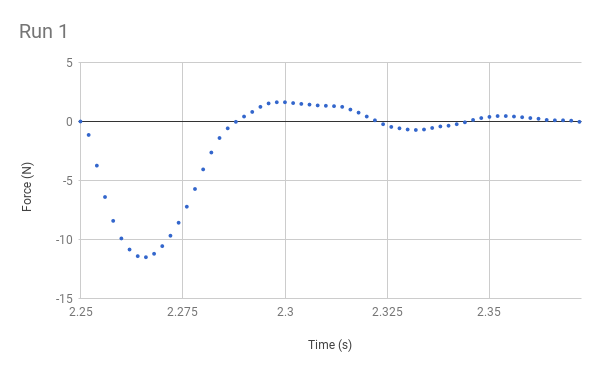
\includegraphics[scale=0.77]{images/08-impulse/run1.png}
    \end{center}
    \caption{}
    \label{figure.08.run.1}
\end{figure}
%%%%%%%%%%%%%%%%%%%%%%%%%%%%%%%%%%%%%%%%%%%%%%%%%%%%%%%%%%%%%%%%%%%%%%%%%%%%%%%%
\section{Your Data}
%%%%%%%%%%%%%%%%%%%%%%%%%%%%%%%%%%%%%%%%%%%%%%%%%%%%%%%%%%%%%%%%%%%%%%%%%%%%%%%%
You collected data for elastic collisions. Everyone is going to use the same data for the inelastic case.
%%%%%%%%%%%%%%%%%%%%%%%%%%%%%%%%%%%%%%%%%%%%%%%%%%%%%%%%%%%%%%%%%%%%%%%%%%%%%%%%
\section{Your Lab Report}
%%%%%%%%%%%%%%%%%%%%%%%%%%%%%%%%%%%%%%%%%%%%%%%%%%%%%%%%%%%%%%%%%%%%%%%%%%%%%%%%
In your lab report you should include:
\begin{enumerate}
    \item A table like table \ref{table.08.results.elastic} for both the elastic and the inelastic collisions. Use these tables to answer the questions below.
    \item A table like table \ref{table.08.results.inelastic} for both the elastic and the inelastic collisions.
    \item How does the average force during the elastic collisions compare to the average force during the inelastic collision?
    \item How does the collision duration $\Delta t$ for the elastic collisions compare to the inelastic collisions?
\end{enumerate}